\section{Additional Diagnostics (Qualitative Selection Provenance, Training Dynamics, Agreement, Thresholds)}
\label{app:diagnostics}

This appendix collects zero-retraining diagnostics derived from the frozen prediction assets and seed-42 metric histories.
Qualitative grids in the main text use \emph{predefined ranking rules} (not visual cherry-picking); the exact selected paths and scores are archived in the repository file \texttt{docs/qualitative\_selection\_meta.json}.

\begin{figure}[H]
\centering
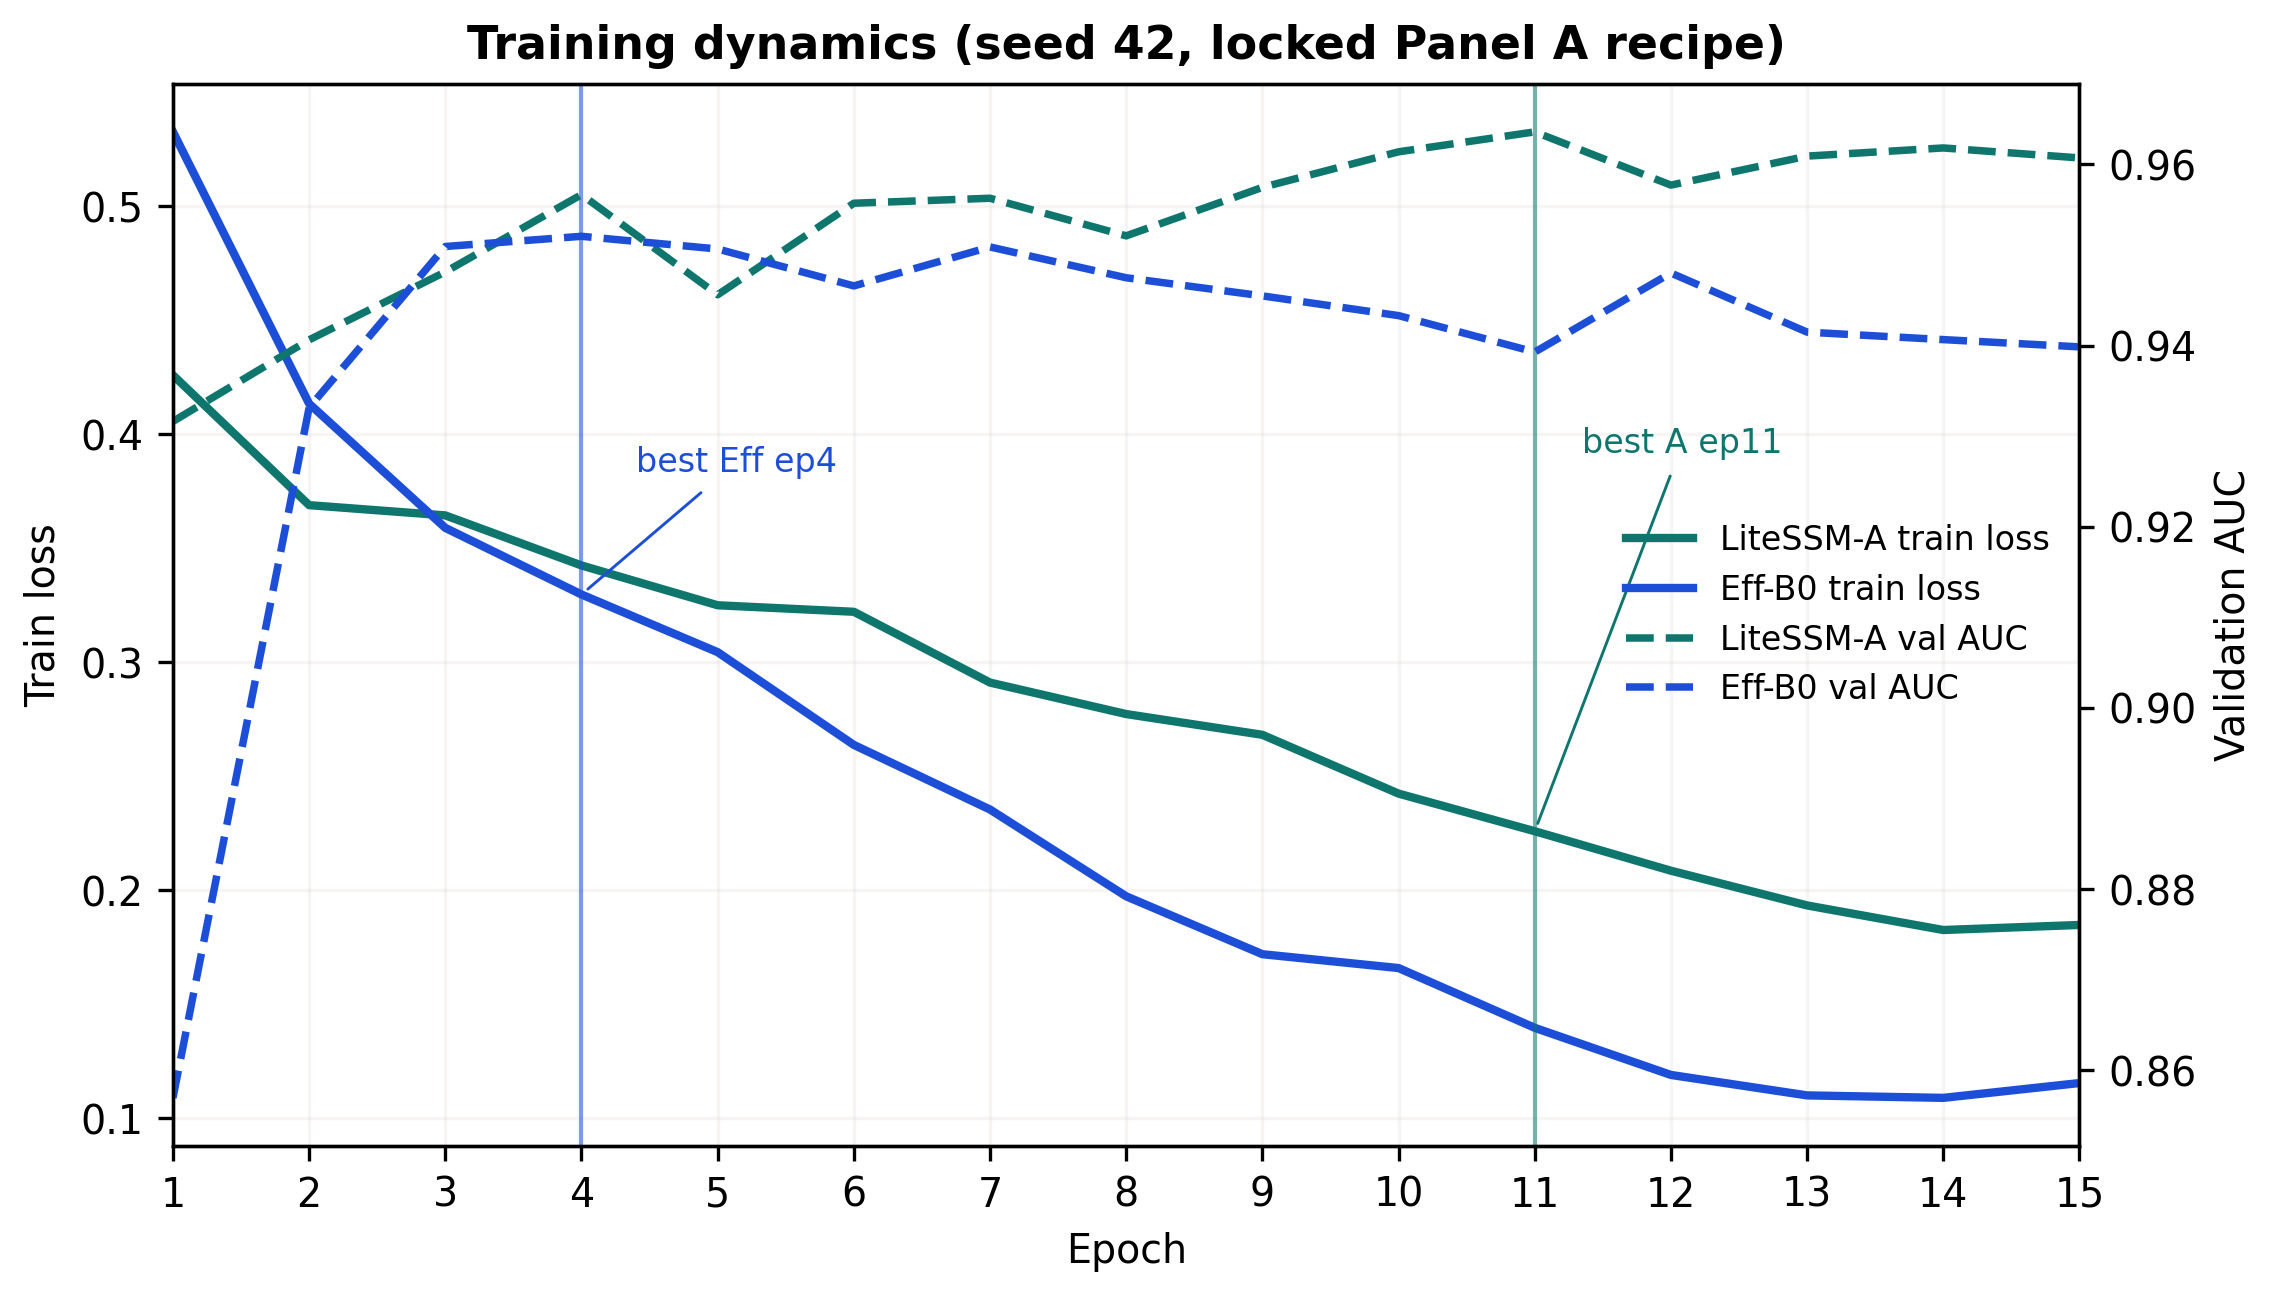
\includegraphics[width=0.92\textwidth]{figures/fig_training_dynamics.png}
\caption{Training dynamics under the locked Panel~A recipe (seed~42, 15~epochs).
Solid lines: train loss (left axis); dashed lines: validation AUC (right axis).
Vertical markers indicate the best-validation-AUC checkpoint epoch used for deployment
(LiteSSM-A: epoch~11; EfficientNet-B0: epoch~4).
Both models stabilize well before epoch~15; EfficientNet-B0 peaks earlier while LiteSSM-A continues to improve validation AUC into the second half of training.\label{fig:train-dyn}}
\end{figure}

\begin{figure}[H]
\centering
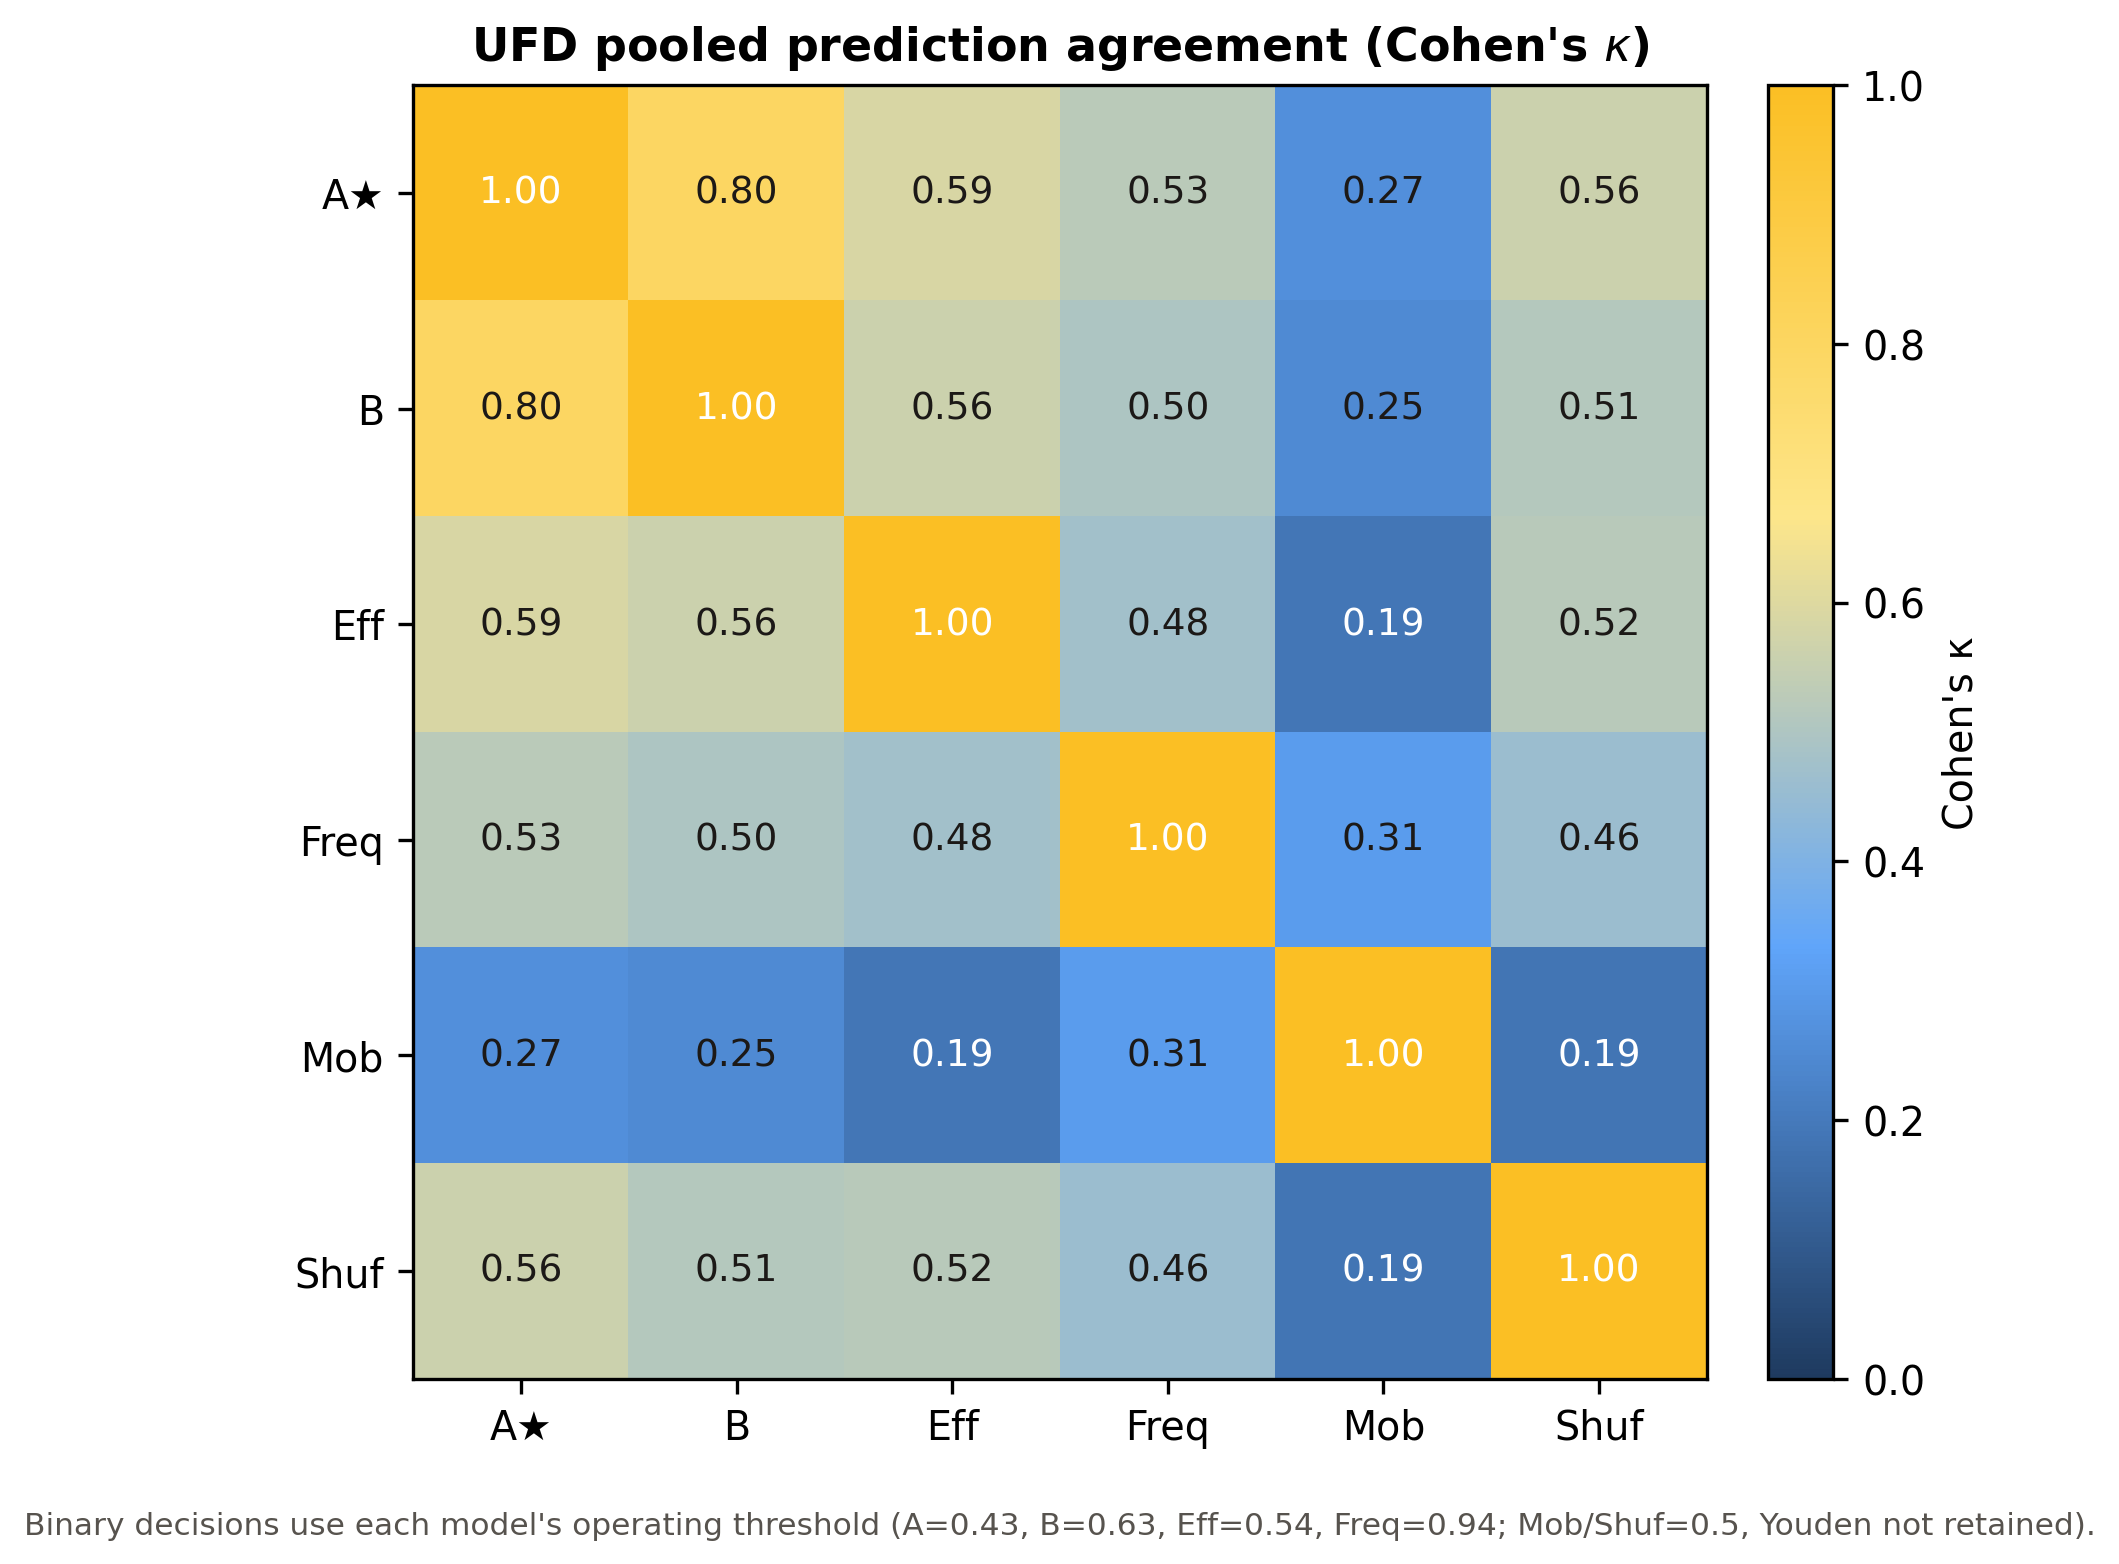
\includegraphics[width=0.78\textwidth]{figures/fig_error_kappa_ufd.png}
\caption{Pairwise Cohen's $\kappa$ among Panel~A binary decisions on UFD (pooled).
High $\kappa$ (yellow) indicates overlapping decisions; low $\kappa$ (blue) indicates complementary errors.
LiteSSM-A/B agree strongly ($\kappa\approx0.80$), while agreement with MobileNetV3-S is much weaker, suggesting that some failures are shared protocol-level blind spots (e.g., DALL·E) rather than a single-architecture artifact.
MobileNetV3-S and ShuffleNet thresholds were not retained in the freeze and use a fixed score threshold of $0.5$ (disclosed on the figure).\label{fig:kappa}}
\end{figure}

\begin{figure}[H]
\centering
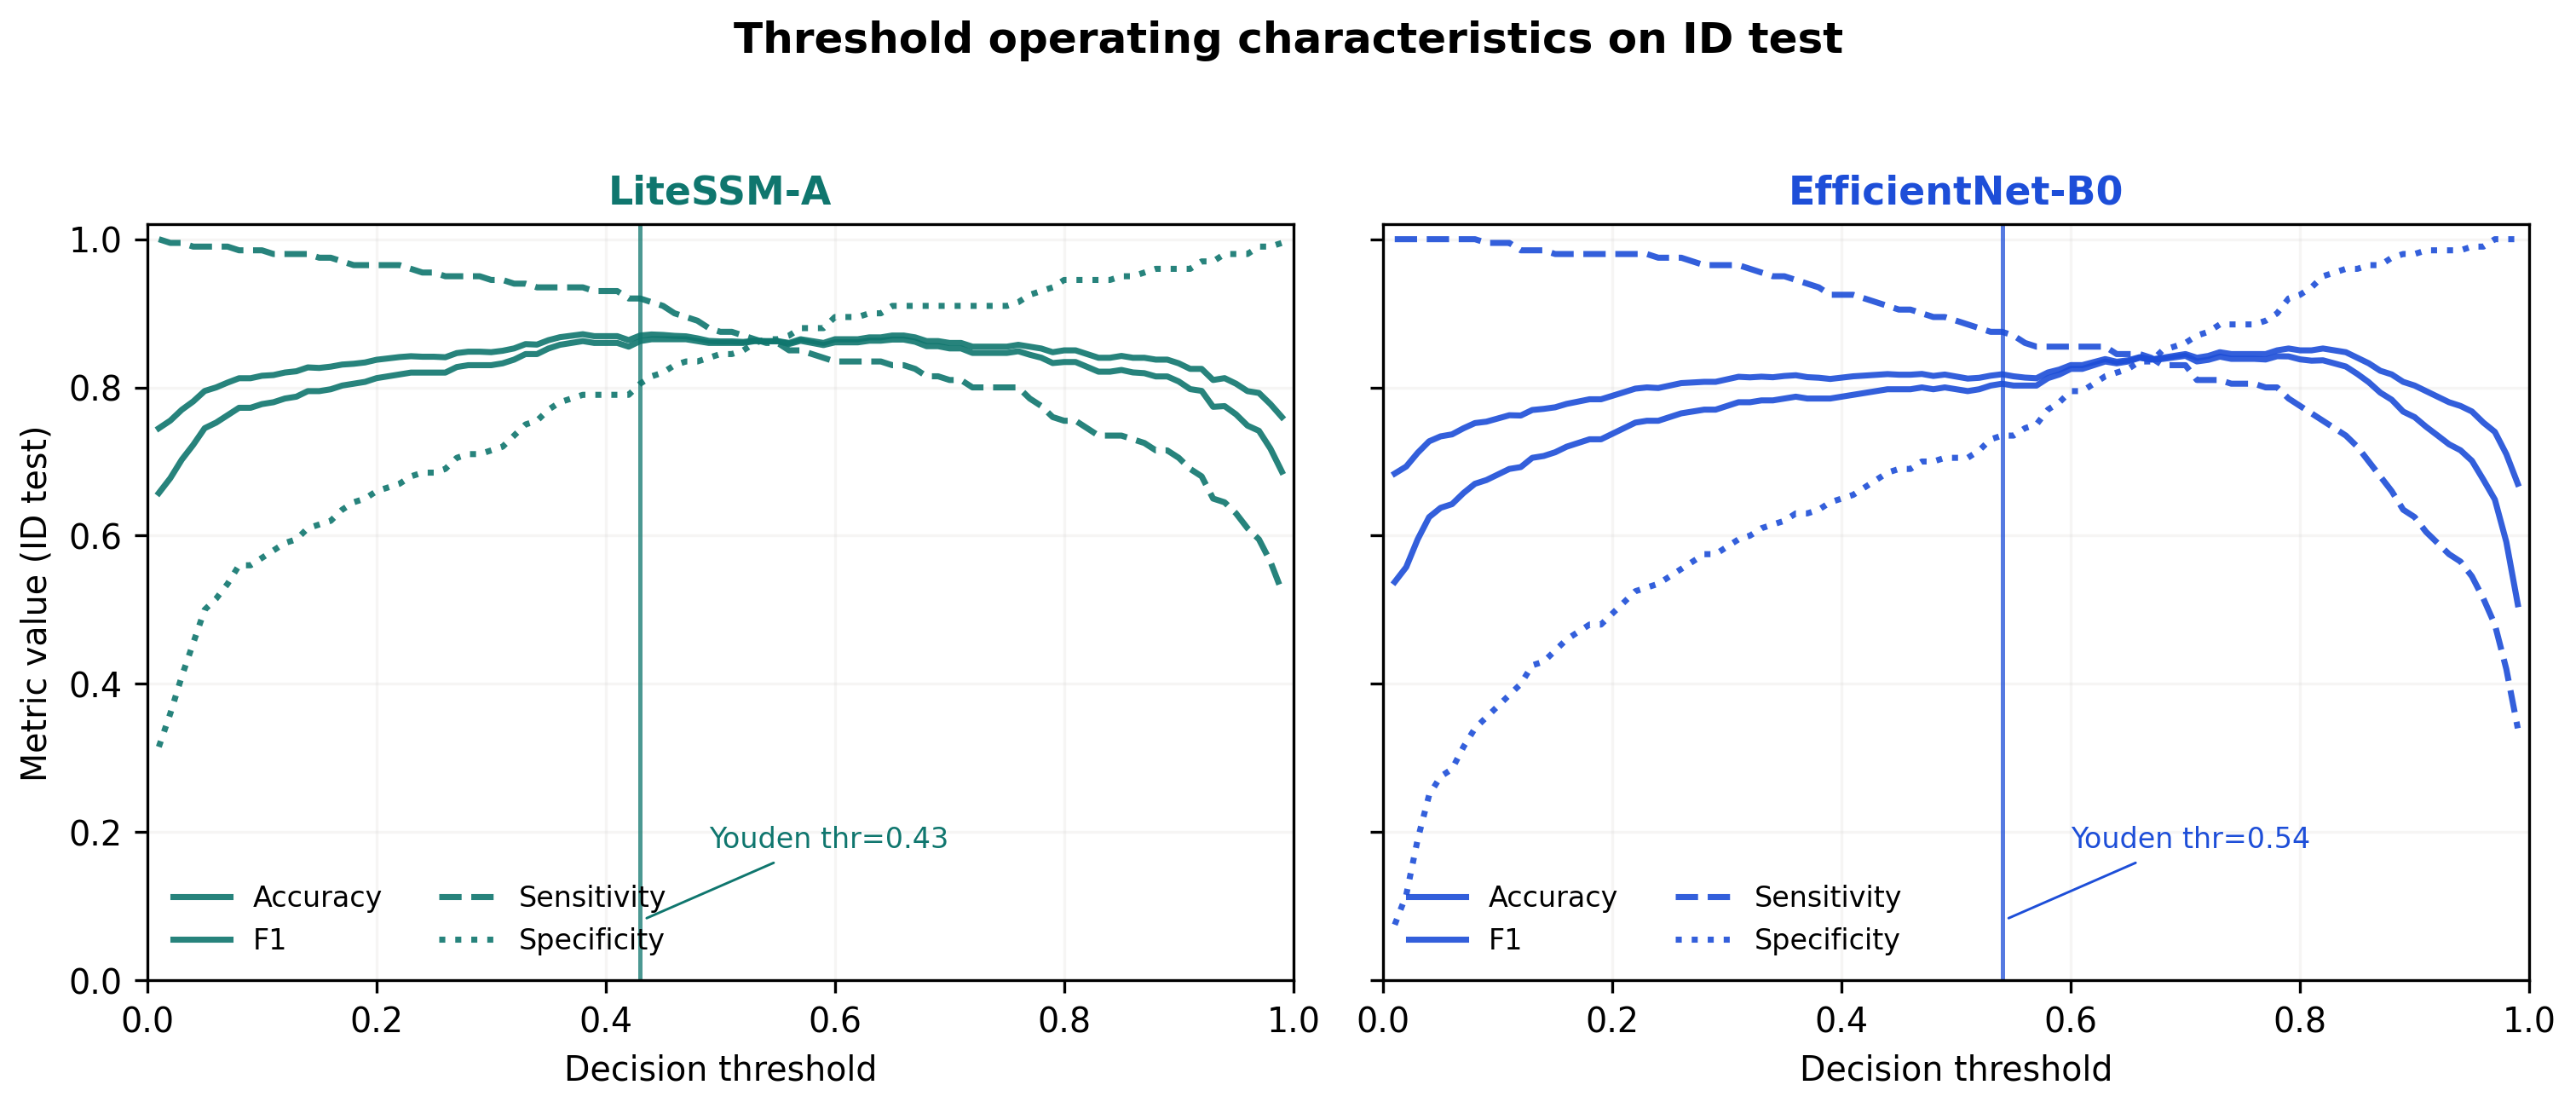
\includegraphics[width=0.96\textwidth]{figures/fig_threshold_sweep_id.png}
\caption{Threshold operating characteristics on the ID test split for LiteSSM-A and EfficientNet-B0.
Curves show Accuracy, F1, Sensitivity, and Specificity versus the decision threshold; vertical lines mark the validation Youden's~$J$ thresholds locked in Table~\ref{tab:operate} (0.43 / 0.54).
Near the selected operating points, Accuracy/F1 form a broad plateau, indicating moderate sensitivity to small threshold perturbations.\label{fig:thr-sweep}}
\end{figure}
